\documentclass{standalone}
\usepackage{mathpazo}
\usepackage[european resistors, american voltages, american currents]{circuitikz}

\begin{document}
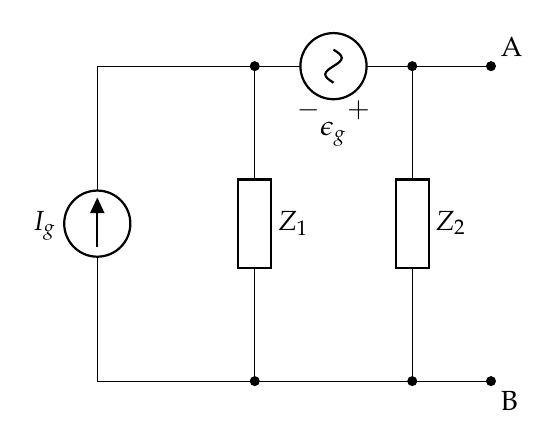
\begin{tikzpicture}
  \coordinate (A) at (0,4);
  \coordinate (B) at (2,4);
  \coordinate (C) at (4,4);
  \coordinate (D) at (5,4);
  \coordinate (E) at (0,0);
  \coordinate (F) at (2,0);
  \coordinate (G) at (4,0);
  \coordinate (H) at (5,0);
  \draw
  (A) to [short, -*] (B)
  (C) to [sV, *-, v=$\epsilon_g$] (B)
  (C) to [short] (D)
  (E) to [short, -*] (F) to [short, -*] (G) to [short] (H)
  (E) to [isource, l=$I_g$] (A)
  (B) to [R, l=$Z_1$] (F)
  (C) to [R, l=$Z_2$] (G)
  (D) node[above right] {A} to [open, *-*] (H) node[below right] {B};
  \end{tikzpicture}
\end{document}